%%-*-latex-*-

\section{Architecture}

Substation Automation Systems (SAS) have a general tendency
within their control system, here, the configuration allows to connect
all the Intelligent Electrical Devices (IED, including protection relays,
numeric transducers, energy meters, monitoring hardware, etc), keeping
field controllers at a level higher than the others
IED~\cite{rodriguez:2007}.

\begin{figure}
  \centering
  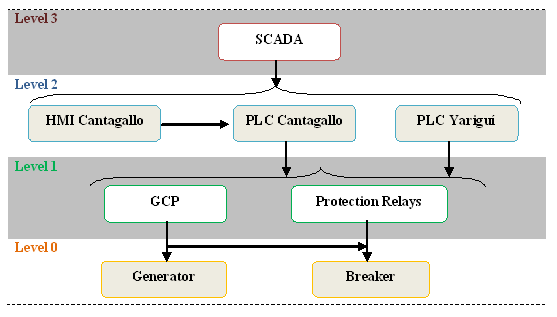
\includegraphics[width=0.5\textwidth]{img/sas.png}
  \caption{Hierarchical structure for the SAS}
  \label{fig:sas}
\end{figure}

\Fig{fig:sas} shows the suggested hierarchical control structure for
generation plants. This has a distributed configuration where hardware
and software are totally integrated to the main communication channel.

The system architecture is based on the automation ideal guidelines,
specifically, in the contemporary approach of automation of electrical
substations. We mainly aim to modularity, robustness and distributed
control. \Fig{fig:arch} shows such architecture and the final system
conception.

In the suggested solution an Ethernet network serves as core for all
the communications, with an 8 ports 100BaseTX switch. Because of the
location conditions broad band Radios were made available. These radios 
were set up in bridge mode using the IEEE 802.11 standard in the 2.46GHz 
band in order to do the remote link between the central control unit at
Yariguí and the electrical substation at Cantagallo. In this way the SAS
creates a virtual single information network in order to share data.

\begin{figure*}
  \centering
  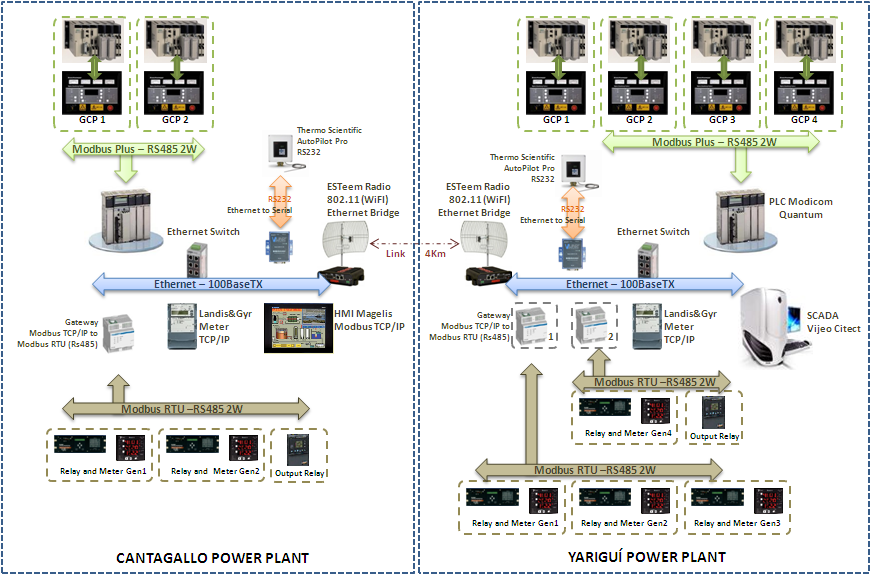
\includegraphics[width=1.0\textwidth]{img/arch.png}
  \caption{System architecture}
  \label{fig:arch}
\end{figure*}

A Modicon Quantum PLC stores data from the generators protection
relays, the output line's bay meters and the protection relay. The PLC
establishes the communication link with a Gateway trough the Modbus
TCP/IP protocol. This is translated to Modbus RTU (with a 2 wires
physical layer RS485) for data acquisition by each hardware that
corresponds to each bay.

At the Cantagallo generation center the Modbus RTU network has 5 nodes
deployed with one gateway. Likewise, the Yariguí generation center 
have two Gateways, one of them  with 6 nodes and the other with 3. 
This is done  in order to get fast data transfer and also for simplicity 
according to the hardware physical disposition.

The generators control units communication is done by the Modbus Plus
between the Quantum PLC and the Premium PLC included at the GCPs made
by Cummins. Only system supervision queries are run trough this bus.
The solution offers, in integrated control, the use of specific
Quantum PLC cards with digital outputs type contactor relay, digital inputs or
analog outputs related to the synchronization controls, start, stops,
trip signals, reset, generators parameters adjustment, etc.

The SCADA system used during the development is Vijeo Citect by
Schneider Electric. This integrates in a simple and fast way every
system communication because of the Modbus predominance with its
several versions installed at the generation center's hardware. The
SCADA operates on a DELL Server offering a stable and reliable
response for control and supervision.

Because the Cantagallo generation center must be remotely operated
an HMI was provided. From there, it is possible to send control
commands and full data supervision when local operation is required,
The HMI is a Magelis Smart tactile screen by the Schneider Electric 
manufacturer.

ThemoScientific gas meters use the Modbus Daniels protocol over a
serial RS232 interface. For this it was necessary to install on each
bus an Ethernet to serial (Serial Server) converter. This allows
multiple TCP connections on the same serial device. The converter
software emulates a virtual serial port enabling the SCADA to directly
consult the gas meter data.

The Landis \& Gyr meter is integrated to the Ethernet network by a
communication module offered by the manufacturer. Finally, The meter
data is collected and stored by the device software.

This way every electronic device within the generation centers is
integrated to the main communication network enabling an effective
solution with stable and reliable links.

